\subsection{.NET Framework}


.NET Framework – программная платформа, от компании Microsoft. Основой платформы является общеязыковая среда исполнения CLR, которая подходит для разных языков программирования. Функциональные возможности CLR доступны в любых языках программирования, использующих эту среду.

Платформа  .NET Framework состоит из двух основных компонентов: среды CLR и библиотеки классов .NET Framework. Среда CLR – это фундамент платформы .NET Framework. Это своеобразный агент, управляющий кодом во время его выполнения, предоставляющий ключевые службы, связанные с такими процессами, как управление памятью, потоками и удаленными операциями, а также обеспечивающий безопасность типов и другими способами контролирующий правильность кода, гарантируя безопасность и стабильность приложений. Понятие управления кодом является для среды основополагающим. Код, созданный для среды, называется управляемым. Любой другой код называется неуправляемым кодом. Библиотека классов, второй основной компонент платформы .NET Framework, является обширным объектно-ориентированным набором типов, которые можно использовать для разработки самых различных приложений – от классических приложений с интерфейсом командной строки или графическим интерфейсом пользователя до новейших приложений на базе технологий ASP.NET, например веб-форм и веб-служб XML.

На следующем рисунке демонстрируется взаимосвязь среды CLR и библиотеки классов с пользовательскими приложениями и всей системой. На рисунке также показано, как управляемый код работает в пределах более широкой архитектуры.

\begin{figure}[h!]
	\centering
	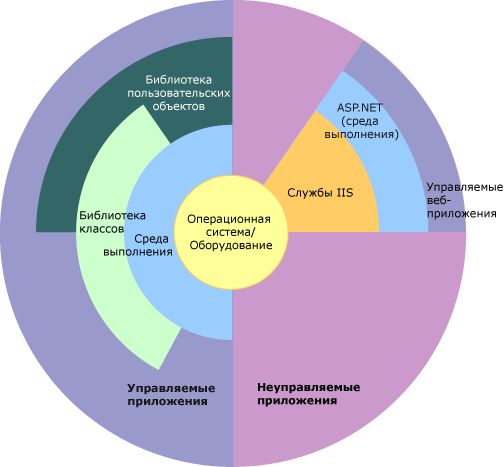
\includegraphics[scale=0.78]{circle.png}
	\caption{Платформа .NET Framework в контексте}
\end{figure}
